% Metódy inžinierskej práce

\documentclass[10pt,twoside,slovak,a4paper]{article}

\usepackage[slovak]{babel}
%\usepackage[T1]{fontenc}
\usepackage[IL2]{fontenc} % lepšia sadzba písmena Ľ než v T1
\usepackage[utf8]{inputenc}
\usepackage{graphicx}
\usepackage{url} % príkaz \url na formátovanie URL
\usepackage{hyperref} % odkazy v texte budú aktívne (pri niektorých triedach dokumentov spôsobuje posun textu)



\usepackage{cite}
%\usepackage{times}

\pagestyle{plain}

\title{Hry o prežitie\thanks{Semestrálny projekt v predmete Metódy inžinierskej práce, ak. rok 2022/2023, vedenie: Vladimír Mlynarovič}} % meno a priezvisko vyučujúceho na cvičeniach

\author{Vojtech Babinský\\[2pt]
	{\small Slovenská technická univerzita v Bratislave}\\
	{\small Fakulta informatiky a informačných technológií}\\
	{\small \texttt{xbabinskyv@stuba.sk}}
	}

\date{\small 6. november 2022} % upravte



\begin{document}

\maketitle

\begin{abstract}

Vďaka pokroku, sa už väčšina populácie v rozvinutých krajinách nemusí zaoberať poľnohospodárstvom, lovom, zberom a podobnou ťažkou fyzickou prácou. Tieto aktivity, dnes vykonáva, vzhľadom na ostatok obyvateľstva, len hŕstka ľudí. 

Niektorí ľudia, však vo svojom voľnom čase siahajú po hrách simulujúcich tieto činnosti, často v extrémnych podmienkach, kde každá chyba môže mať nemilý vplyv na ďalšie hranie. Ide teda o špecifický prípad, kde na rozdiel od väčšiny iných hier, hráč nie je nezraniteľným hrdinom, ale súčasťou prostredia, v ktorom zápasí s hladom, zvieratami/príšerami, počasím, inými hráčmi atď. 

Cieľom článku je zoznámiť čitateľa s tzv. hrami o prežite (ang. Survival games).Pokúsi sa opísať kritéria, ktoré musia hry spĺňať, aby mohli byť zaradené do tohto žánru, poskytne príklady  úspešných herných predstaviteľov tejto kategórie a predstaví aj jej rôzne subžánre. 
\end{abstract}


\newpage

\section{Úvod}
Počítačové hry sú relatívne nová forma zábavy, ktorej vývoj kopíruje rozvoj a dostupnosť počítačov. Tak ako v literatúre, jestvuje mnoho rozličných žánrov. Hranice medzi žánrami hier sú pružné, niektoré hry teda môžu mať znaky viacerých naraz. V tomto článku sa budem zaoberať „hrami o prežitie“ (alebo aj survival hry ). 

Ako už napovedá sám názov tohto druhu hier, hlavným cieľom hráča je prežiť. Základnou črtou survival hier je hospodárenie so surovinami, často zahrňujúce výrobu (crafting) a recykláciu, pomocou, ktorých dokážete svoju postavu dlhšie udržať pri živote. \cite{Pavlovic}

Ďalším znakom je možnosť zranenia sa (prejavuje sa ako dočasné znevýhodnenie hráča), prípadne smrti v hre. 

Taktiež, konfrontácia s inými ľuďmi, zvieratami a príšerami patrí medzi základne elementy hier o prežitie.\cite{Reid}


\section{História hier o prežitie }

\begin{figure}[h]
	\begin{flushleft}
		
		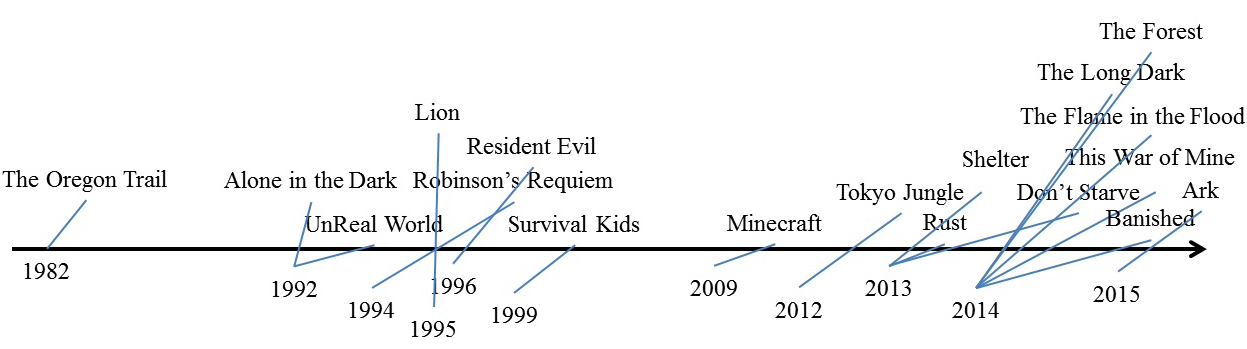
\includegraphics[width=12.5cm,keepaspectratio]{REID_graf.png}
		\caption{\textit{Časová os vzniku žánru videohier s tematikou prežitia}}
\label{ fig:Časová os vzniku žánru videohier s tematikou prežitia}
		
	\end{flushleft}
\end{figure}

Prvou komerčne úspešnou survival hrou bola The Oregon trail, vydaná v 80tych rokoch minulého storočia, jej úplne prvá verzia, však uzrela svetlo sveta v roku 1971. 

Dan Rawitsch, vtedy 21 ročný vysokoškolák a učiteľ , dostal za úlohu učiť žiakov 8. triedy históriu americkej expanzie na západ. Chcel urobiť niečo nové a interaktívne, a preto pre svojich žiakov vytvoril stolnú hru. \cite{Toppo}

Keď jeho spolubývajúci, učiteľ matematiky,  Bill Heinemann videl mapu tejto hry povedal Rawitschovi, že by to mohol byť perfektný program pre počítač. Ukázal mapu ďalšiemu spolubývajúcemu Paulovi Dillenbergerovi, ktorý tiež učil matematiku. Tomu sa nápad zapáčil a pustili sa do diela. 

Základ hry je cestovanie so skupinkou osadníkov z mestečka Independence (štát Missouri) do štátu Oregon na východe  USA.

V úvode si hráč nakúpi zásoby jedla, náboje a zvieratá na cestu.  Počas výpravy musí prekonať rôzne náhodné udalosti ako rozbitie kolesa na voze, uhryznutie hadom a choroby.

Hra nemala žiadnu grafiku a bola čisto textová, jej kód mal 800 riadkov a bola naprogramovaná v jazyku BASIC. Ihneď sa stala hitom medzi študentmi školy, ktorí stáli v radoch aby si mohli zahrať. 

Hoci po vydaní The Oregon Trail nasledovala dekáda útlmu popularity survival hier \ref{ fig:Časová os vzniku žánru videohier s tematikou prežitia},tento žáner prešiel obrovským vývojom a dnes patrí medzi najobľúbenejšie. \cite{IGN}


\section{Subžánre} 
Survival hry majú dva hlavné subžánre – Wilderness survival (prežitie v divočine) a Survival  horror.  Samozrejme, jestvuje mnoho hier, pri ktorých nie je jednoduché zaradiť ich do jednej z dvoch predstavených skupín, voláme ich preto vznikajúce typy (alebo aj hybridy).

\subsection{Wilderness survival}

Hry tohto subžánru, sa sústredia na schopnosti prežitia v prírode. Hráč zvyčajne musí začať ako lovec a zberač. Postupným hraním si vylepší vybavenie a nájde úkryt, z ktorého vychádza na výpravy. Do tejto skupiny hier patrí napríklad už spomenutá The Oregon Trail, The Long Dark a Unreal World.

\subsubsection{UnReal world}
Prvýkrát vyšla v roku 1992. Je to práca dvoch ľudí, hlavného vývojára Samiho Maaranena a Errku Lehmusa. Pôvodne to bola fantasy RPG hra, ktorá sa postupne vyvinula na Wilderness survival situovaný v dnešnom Fínsku v dobe železnej. 

Hráč sa pohybuje v masívnom náhodne generovanom svete s jediným cieľom, prežiť čo najdlhšie. Pre vysoký level realizmu to vôbec nie je jednoduché. 

UnReal world je držiteľom dvoch rekordov: je to najdlhšie podporovaná hra na svete a prvá survival hra s otvoreným svetom. \cite{UnRealWorld}

\subsubsection{The Long Dark}

Táto kanadská hra z roku 2014, sa odohráva v zimnej a drsnej kanadskej divočine. The Long dark má survival mód a príbehový mód. 

V survival móde ide iba o prežitie, ide o sandbox  mód (hráč má voľnú ruku v tom ako chce hrať). Cieľ tohto módu je prežiť čo najdlhšie.

V príbehovom móde sa hráč sa vtelí do pilota Willa Mackenzieho, ktorý hľadá doktorku Astrid Greenwoodovú, s ktorou stratil kontakt pri záhadnom páde ich lietadla. Až pri nájdení mestečka Milton  si hrdina začne uvedomovať škálu apokalypsy, ktorá postihla svet.\cite{Virtanen}\cite{Reid}

\subsection{Survival Horror}



\subsection{Hybridné žánre}






\section{Záver} \label{zaver} % prípadne iný variant názvu



%\acknowledgement{Ak niekomu chcete poďakovať\ldots}

\newpage
% týmto sa generuje zoznam literatúry z obsahu súboru literatura.bib podľa toho, na čo sa v článku odkazujete
\bibliography{literatura}
\bibliographystyle{plain} % prípadne alpha, abbrv alebo hociktorý iný

\end{document}
